\documentclass[eng]{ajceam-class}
\usepackage{graphicx}
\usepackage{caption}
\usepackage{subcaption}
%
% Publication Title
\title{The Use of Alignment-free Analyses in Predicting the Evolution of Crucivirus}

% Short title for the header (copy the main title if it is not too long)
\shorttitle{Alignment-free Analyses for Predicting Crucivirus Evolution}
       
% Authors
\author[1]{Yuxuan Liu}
\author[2]{Ignacio de la Higuera}

% Author Affiliations
\affil[1]{Institute for Computing in Research}

% Surname of the first author of the manuscript
\firstauthor{Liu, de la Higuera}

%Contact Author Information
\contactauthor{Yuxuan Liu}           % Name and surname of the contact author
\email{liu.family.yx@gmail.com}            % Contact Author Email

% Publication data (will be defined in the edition)
\thisvolume{XX}
\thisnumber{XX}
\thismonth{Month}
\thisyear{20XX}
\receptiondate{dd/mm/aaaa}
\acceptancedate{dd/mm/aaaa}
\publicationdate{dd/mm/aaaa}

% Place your particular definitions here
\newcommand{\vect}[1]{\mathbf{#1}}  % vectors

% Insert here the abstract in English language
\abstract{For a long time, scientists had believed that viruses could only contain RNA or DNA, and never both. However, the discovery of the crucivirus, a type of virus that has the characteristics of circular rep-encoding single-stranded DNA virus but also carry a capsid gene that is similar to the capsid gene of RNA tombusvirus, made people turn over the previous predictions about virus evolution. What is the relationship between crucivirus and the viruses that only have DNA or RNA? In this project, we will investigate the evolution of crucivirus as well as its relations with DNA and RNA viruses through four alignment-free analyses: genome sense prediction, pairwise comparison, k-mer similarity between CP and Rep genes, and comparison of k-mer between genomes. Genome sense prediction helped identify genomes that had recently undergone horizontal genetic transfer. Pairwise comparison helped find the different processes of evolution between the CP and Rep genes of the same crucivirus genome and found two genomes, \texttt{Cruci\_CruV\_319} and \texttt{Cruci\_CruV\_320}, that may have recently diverged from their closest common ancestor. K-mer similarity between CP and Rep genes helped us compare the similarity between CP and Rep of crucivirus, DNA virus, and RNA virus. Finally, comparison of k-mer between genomes, specifically between DNA virus and crucivirus, showed possible locations of horizontal genetic transfer between DNA virus and crucivirus.}

% Insert here the keywords of your work in English language
\keywords{
Virus, Evolution, Nucleotide, Crucivirus, alignment-free}

% Start document
\begin{document}

% Include title, authors, abstract, etc.
\maketitle
\thispagestyle{fancy}
\printcontactdata

% Main body of manuscript
\section{Introduction}
\firstword{V}{iruses}% Capital letter in first word
are often seen as microscopic non-living organisms and pathogens that spread diseases and start pandemics. Yet, these small bundles of nucleotides play a crucial role in the evolution of all organisms on Earth. As they jump from one infected organism to the other, they carry and spread the genetic materials they grabbed from their past hosts’ DNA to their new hosts. Not only do they push the evolutionary process of their hosts, but viruses also exchange genetic materials amongst themselves, forming a wide variety of species over time [1]. 

Viruses hold many forms, but all consist of nucleic acid and a protein shell called capsid. Because of their simple structures, viruses are not able to sustain life-sustaining functions and reproduction independently. Viruses get energy and other metabolic functions, and basic building materials such as amino acids from their host cell. They also use the ribosomes of their hosts to generate proteins and replicate within the infected cell. The dependency of viruses on their host to reproduce and carry important functions causes them to not be considered living organisms [2].

Although people have identified many properties of viruses, viruses and their evolutionary process are still mysterious and yet to be unveiled. Until recently, scientists had only found viruses containing either DNA or RNA, but never both. They believed that viruses could only be made of DNA or RNA. Yet, the discovery of of crucivirus - a virus that has both the characteristics of circular rep-encoding single-stranded DNA virus (CRESS DNA-virus) and a capsid-encoding gene that resembles the reverse transcription of capsid genes found in RNA tombusviruses [3] - overturned this idea. Since the first discovery of crucivirus in 2012 by the Stedman lab at Boiling Springs Lake, Lassen Volcanic National Park, hundreds of sequences of CruV virus have been identified in a variety of environments around the world. The discovery of crucivirus brought new questions to the field of microbiology [4]. Where did crucivirus acquire its capsid gene? Did it grab the gene from a RNA virus? Is crucivirus a result of horizontal genetic transfer between DNA virus and RNA virus, with the DNA virus receiving the capsid from the RNA virus, or is crucivirus older than the two widely known virus types and that both DNA and RNA had evolved from crucivirus? Researchers have done many types of analyses to understand the evolution of crucivirus, with the main ones being phylogenetic and network analyses. In this project, we used a type of analysis called alignment-free analysis to find clues to the history of crucivirus. 

Alignment-free methods are widely characterized to use subsequences and be based on the subsequence length. Subsequences are often referred to as k-mer or n-grams, with k and n representing the length of the subsequences. K-mers are taken from a sequence through the concept of the sliding-window. Every time a window of length k slides one nucleotide across a sequence of nucleotides, a new k-mer is shown. Adjacent k-mer sequences overlap by n >= 1, with n typically k - 1 [5]. In this project, we found k-mers that slide over 1 nucleotide with each k-mer and overlap adjacent k-mer by k - 1. alignment-free analyses may provide great insight in the relationship of crucivirus with DNA and RNA viruses, cruciviruses with each other, and capsid and replication genes. Findings that sequences share k-mers may indicate that they are homologous if the k-mers follow certain criteria. For example, k-mer sequences that appeared at high frequency in two sequences infer that the two sequences may have crossed paths in evolution. Sequences that share large k-mers may indicate genetic transfer because sufficiently large k-mers are considered approximately unique [5]. We employed some alignment-free analyses such as the ones briefly mentioned in this section of our project to predict the evolution of crucivirus and its relationship with other cruciviruses and DNA and RNA viruses.

\section{Methods and Materials}

We used the Linux operating system. All of the programs were written on the Visual Studio Code platform in Python. Python libraries that we used are numpy and pandas, which we installed on the terminal using the pip command line. The graphs are drawn mainly using the Matplotlib library but we also used Scipy and Seaborn to draw the dendrograms and heatmaps respectively. 

We employed four alignment-free methods, which we tested on datasets of crucivirus, DNA virus, and RNA virus genomes and genes. The datasets are written as fasta files. In order to incorporate them into our programs, we wrote a function called readFasta() that converts a fasta file into a python dictionary in the format: gene name/genome name: genetic sequence.

\subsection{Genome Sense Prediction}

First, we wrote a geneStrandPrediction() function that finds the codon-ending preference of a gene. We then wrote a geneStrandsPrediction() function that finds the codon-ending preferences for all genes in a dataset with each gene using geneStrandPrediction(). The geneStrandsPrediction() function gives us the codon-ending preferences for both the CP and Rep genes, which we used in genomeSensePrediction() function to predict the sense of genomes. The results, the genome name, CP codon-ending bias, Rep codon-ending bias, and genome sense are all sorted into a matrix made by genomeSenseTable(). The actual genome senses are in a csv. file. We retrieved the data using readCSV() and compared the predictions with the actual genome senses using checkPrediction(). This gives us the accuracy of our program and the incorrect predictions. The incorrect predictions are arranged into an array of genome names. In order to find the percentage of codons ending in adenine and the percentage of codons ending in thymine of each genome, we wrote the function genomeSenseSurprising(). The function finds the genomes with significant differences between the percentage of nna and the percentage of nnt and are unpredictable.

\subsection{Pairwise Comparison}

We wrote two functions. The first function is pairwise(). It prompts for a dataset of either CP or Rep genes and the length of k-mer. It creates a matrix that consists of the percentages of matching k-mers of all possible pairs in the dataset. The function pairwiseVisual() creates a heatmap and dendrogram using the matrix.

\subsection{K-mer Similarity between CP and Rep genes}

First of all, we wrote a function CPRepKmerCompareRank() that creates a rank containing the percentage of similar k-mers between each pair of CP and Rep based on genome from the pair with the highest similarity to the pair with the lowest similarity. The kmerRankShaded() function finds all the percentages and their corresponding count. The data is visualized in the form of line graphs using the function kmerCPRepVisual(). The data for all three virus types are put in the same graph using the kmerCPRepCompareVisual() function.

\subsection{Comparison of K-mer between Genomes}

First, in order to find the percentage of matching k-mers between genomes, we wrote virusKmerMatch(), which gives a matrix that includes all of the percentages of matching k-mers for pairs of genomes. This data is shown as a heatmap by using the function virusKmerVisual(). The genome pairs with the highest and lowest similarities can be observed and selected from the heatmap. The chosen genome pairs are analyzed to find their matching k-mers and the number of times that the k-mers appeared in both genomes using the functions kmerSequence() and genomeskmerMatch(). The function genomeskmerMatchVisual() uses the data to create a bar graph that shows the shared k-mers and the counts.

\section{Results}

\subsection{Genome Sense Prediction}

\textbf{Table 1.} Genome-sense prediction uses the codon-ending bias of a genome’s genes (capsid protein gene and replication protein gene) to predict the sense or orientation of the genome. If the CP and Rep genes have matching codon-ending bias (both prefer adenine or thymine), the genome is classified as unisense. If the CP and Rep genes have complementary codon-ending bias (one has an overrepresentation of adenine the other thymine), the genome is ambisense [6]. Genes that exist in the same virus accumulate mutations over time. When a genetic strand is recently received by a virus, it does not exhibit the characteristics of the other genes and has not yet accumulated enough mutations to have the characteristics. This creates an unexpected genome sense of the virus. Thus, when we find genomes with senses that do not match the predicted genome senses, we may infer that a horizontal genetic transfer has occurred recently between the genome and another genome. For this method, we used datasets of crucivirus genomes and their capsid and rep genes. We found the codon-ending preference of the capsid and rep of each genome and predicted the genome sense. We then compared our prediction to the actual genome sense. After all of the genomes are predicted using a computer program, we identify the incorrect predictions and filter out the genomes that are incorrectly predicted due to computational errors and limitations (please refer to Limitations). The genomes, just like the correctly predicted genomes, have a significant overrepresentation of a certain codon-ending nucleotide for both its genes but the predictions are different from the actual results. Hence, we propose that these genomes may have contradicting predictions and actual results because of recent horizontal genetic transfers.

\begin{table}
\begin{center}
\scriptsize
\begin{tabular}{||c c c c||}
    \hline
    Genome & CP & Rep & Genome Sense \\ [0.5ex]
    \hline\hline
    \texttt{Cruci\_EAMS\_Lach\_SydneyBayRA1\_c205} & T & T & unisense \\
    \hline
    \texttt{Cruci\_ETS\_Han\_JilinP\_c180} & A & A & unisense \\
    \hline
    \texttt{Cruci\_ETS\_Han\_JilinP\_c180} & A & A & unisense \\
    \hline
    \texttt{Cruci\_NW\_Brin\_10C\_c183} & T & A & ambisense \\
    \hline
    \texttt{Cruci\_EAF\_Roux2\_virusbaton\_c1503} & A & A & unisense \\
    \hline
    \texttt{Cruci\_ETS\_Yu\_ecotone539\_c44} & T & A & ambisense \\
    \hline
    \texttt{Cruci\_ETS\_Han\_JilinP\_c441} & A & T & ambisense \\
    \hline
    \texttt{Cruci\_NW\_Brin\_100B\_c95} & T & A & ambisense \\
    \hline
    \texttt{Cruci\_EAF\_Carc\_IR2\_c6} & A & A & unisense \\
    \hline
    \texttt{Cruci\_EAF\_Colo\_spring\_c82} & A & T & ambisense \\
    \hline
    \texttt{Cruci\_EAF\_Carc\_IR2\_c6} & A & A & unisense \\
    \hline
    \texttt{Cruci\_EAF\_Colo\_spring\_c82} & A & T & ambisense \\
    \hline
    \texttt{Cruci\_EAF\_Colo\_spring\_c82} & A & T & ambisense \\
    \hline
    \texttt{Cruci\_EAF\_Carc\_IR1\_c397} & T & T & unisense \\
    \hline
    \texttt{Cruci\_EAF\_Carc\_IR2\_c14} & T & A & ambisense \\
    \hline
    \texttt{Cruci\_EAF\_Carc\_IR2\_c56} & T & T & unisense \\
    \hline
    \texttt{Cruci\_EAF\_Carc\_IR2\_c60} & T & T & unisense \\
    \hline
    \texttt{Cruci\_EAF\_Carc\_IR2\_c61} & T & A & ambisense \\
    \hline
    \texttt{Cruci\_EAF\_Carc\_IR2\_c103} & T & T & unisense \\
    \hline
    \texttt{Cruci\_EAF\_Carc\_IR2\_c121} & T & T & unisense \\
    \hline
    \texttt{Cruci\_EAF\_Carc\_IR2\_c381} & A & T & ambisense \\
    \hline
    \texttt{Cruci\_EAF\_Carc\_IR2\_c1026} & T & A & ambisense \\
    \hline
    \texttt{Cruci\_EAF\_Carc\_IR2\_c1240} & T & T & unisense \\
    \hline
    \texttt{Cruci\_EAF\_Carc\_IR2\_c1240} & T & A & ambisense \\
    \hline
    \texttt{Cruci\_EAF\_Carc\_IR2\_c1314} & T & T & unisense \\ [1ex]
    \hline
\end{tabular}
\caption{The first 25 crucivirus genomes that we predicted the sense of. The columns shows the genome name, the codon-ending preference of the CP gene, the codon-ending bias of the Rep gene, and the genome sense respectively.}
\end{center}
\end{table}

We tested our program on 945 crucivirus genomes. There is a 70.01\% accuracy in predictions; approximately 70.01\% of the predictions are correct. Out of the 274 genomes incorrectly predicted, 119 of them are considered to have unexpected genome senses. This is determined by differences between percentages of thymine-ending codons (nnt) and percentages of adenine-ending codons (nna) that are greater than 0.05 for both CP and Rep genes. The rest of the incorrect predictions have very close percentages of nnt and nna for either both or one of the genes. This is further explained in Limitations. The genomes with unexpected senses may have had horizontal genetic transfer recently.

\subsection{Pairwise Comparison}

Pairwise comparison compares every sequence of a dataset with each other, including with itself. We used this method to compare the composition of shared k-mer of crucivirus capsid genes and rep genes. We used two datasets, one for the capsid genes and the other for rep. We calculated the percentage of matching k-mer with k = 7 for all possible pairs of genes within each dataset. The percentages are used to examine patterns and relationships between capsid genes and rep genes of cruciviruses. Genes with similar k-mer composition have closer common ancestors. This can help us predict the evolution of crucivirus capsid genes and the evolution of crucivirus replication genes and analyze if there are intersections throughout the evolutionary processes of the two genes. We may use these results to predict if and for how long capsid and rep genes have coexisted in crucivirus.

\begin{figure}
    \centering
    \textbf{Pairwise Comparison of Capsid Genes}\par\medskip
    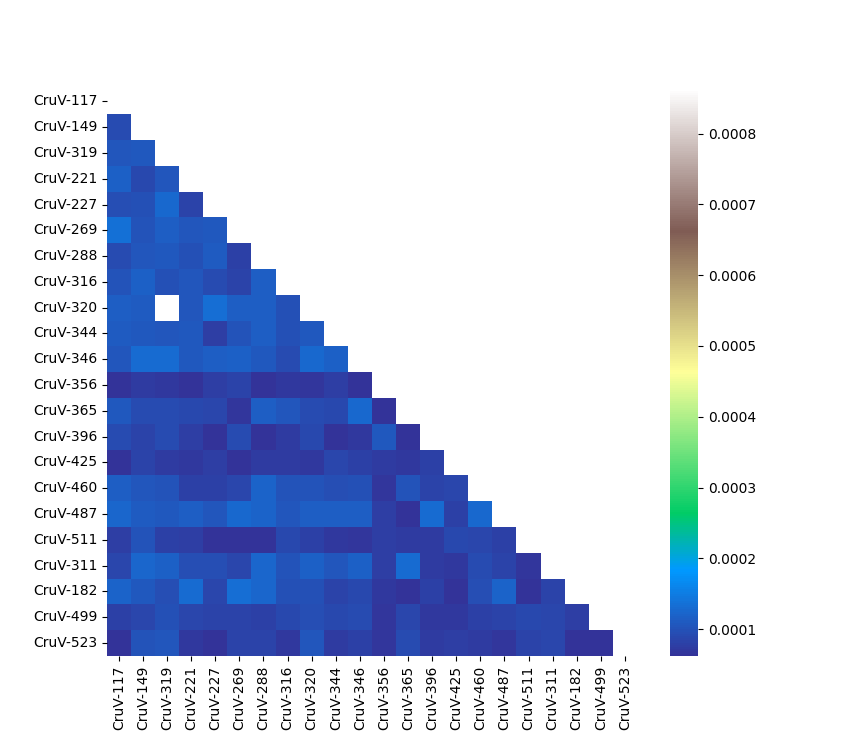
\includegraphics[scale=0.4]{PairwiseCPHeatmap.png}
    \caption{22 crucivirus capsid genes are paired with each other, including with themselves. Each cell represent the percentage of shared k-mers, with k = 7, for the CP genes pair with the same names as the cell coordinates.}
\end{figure}

\begin{figure}
    \centering
    \textbf{Pairwise Comparison of Replication Genes}\par\medskip
    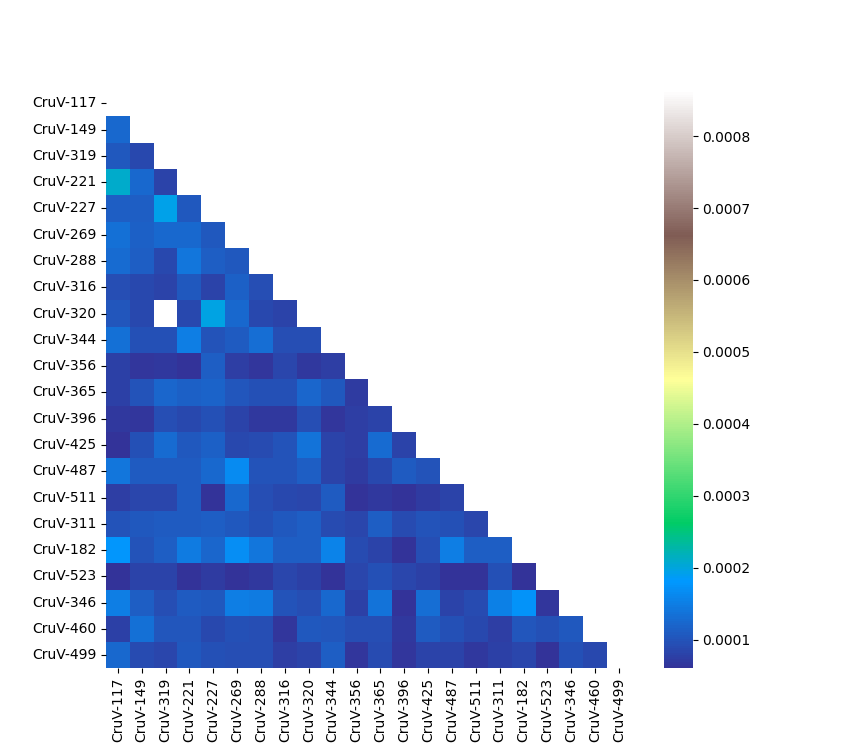
\includegraphics[scale=0.4]{PairwiseRepHeatmap.png}
    \caption{22 crucivirus capsid genes are paired with each other, including with themselves. Each cell represent the percentage of shared k-mers, with k = 7, for the Rep genes pair with the same names as the cell coordinates.}
\end{figure}

\begin{figure}
    \centering
    \begin{subfigure}[h]{0.5\textwidth}
        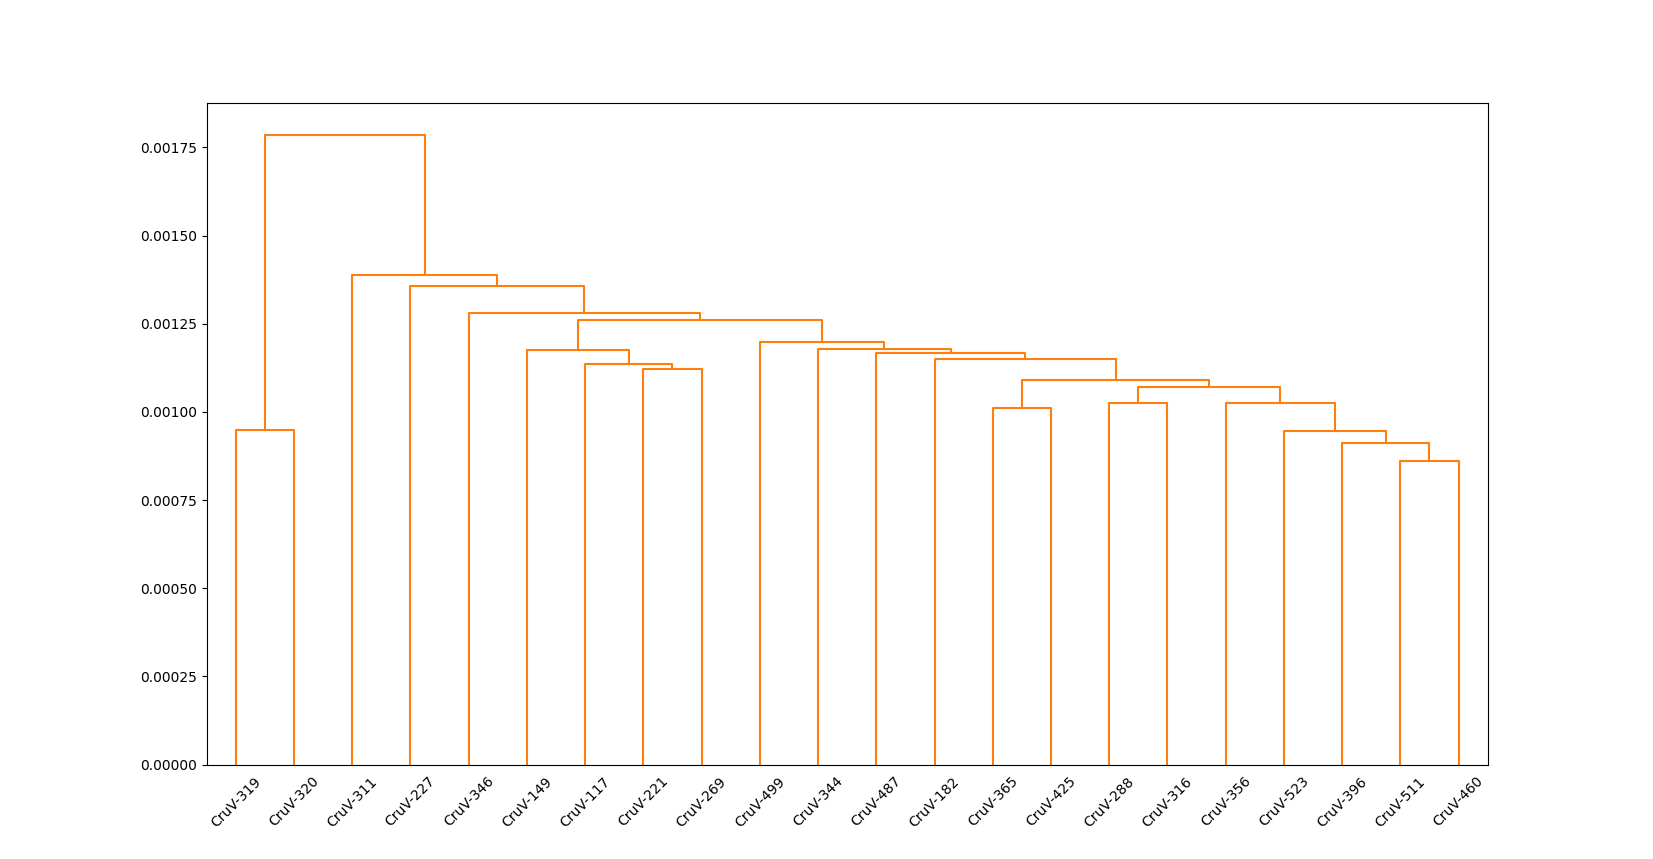
\includegraphics[width=\linewidth]{PairwiseCPDendrogram.png}
    \end{subfigure}
    \hfill
    \begin{subfigure}[h]{0.5\textwidth}
        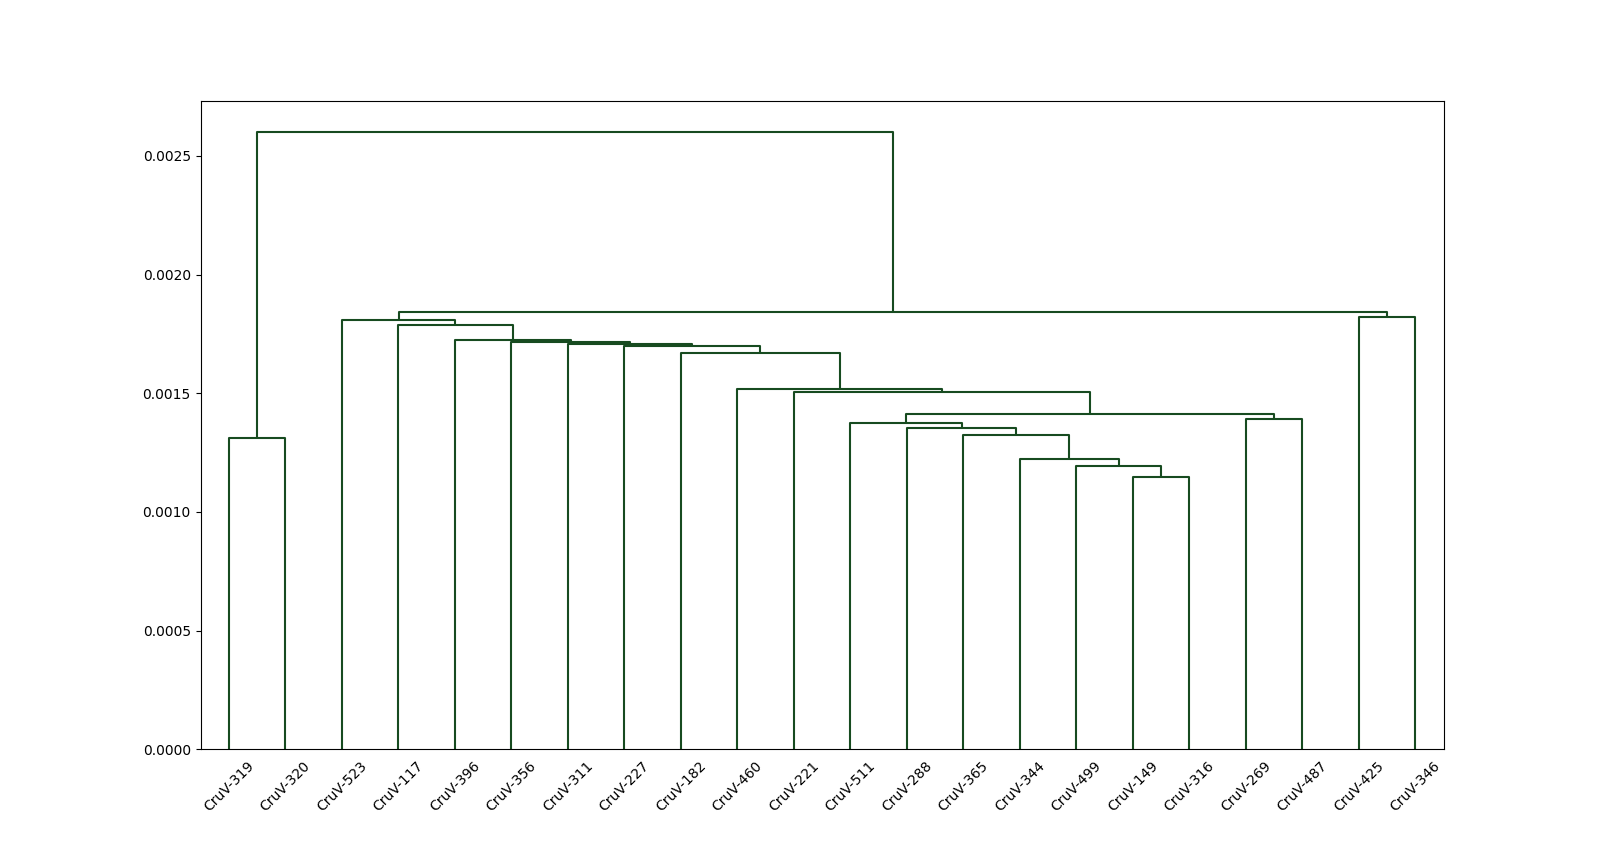
\includegraphics[width=\linewidth]{PairwiseRepDendrogram.png}
    \end{subfigure}
    \caption{Top: Capsid genes are clustered based on the percentage of shared k-mers between genes. Genes with greater similarities are closer to each other. Bottom: Replication genes are clustered based on the percentage of shared k-mers between genes. Genes with greater similarities are closer to each other.}
\end{figure}
\textbf{Figure 1.} The cells on the diagonal line have relatively light colors compared to other cells. The line represents the percentages of gene pairs with identical genes, thus having the highest similarities. The reason why the similarity is not 1.00 is that all k-mers are compared to all k-mers and not in the order of the nucleotide sequences. The cells representing genes compared to genes that are not themselves are usually a shade of blue, which is a range of similarity between 0.0001 and 0.0002. There is an exception at the cell with coordinates \texttt{Cruci\_CruV\_319} and \texttt{Cruci\_CruV\_320}. The cell is white, contrasting strongly from the surrounding cells, and has a percentage of similar k-mers larger than 0.0008. \textbf{Figure 2.} The heatmap for rep genes gives similar results. The diagonal line of pairs with the same genes has the highest similarities and brightest colors. Most of the other cells have shades of blue and have low similarities. \texttt{Cruci\_CruV\_319} and \texttt{Cruci\_CruV\_320} have a white color, meaning that the Rep genes of the two genomes have a similarity higher than 0.0008. \textbf{Figure 3.} The dendrograms for CP and Rep also show that the CP and Rep genes of \texttt{Cruci\_CruV\_319} and \texttt{Cruci\_CruV\_320} are closer to each other than to any other genes. 

The data suggest that \texttt{Cruci\_CruV\_319} and \texttt{Cruci\_CruV\_320} probably have only recently diverged from each other and are located close to each other in the phylogenetic tree because the similarities of k-mers between their CP genes and Rep genes are so high. As shown on the dendrograms, most of the CP and Rep have different predicted evolutionary paths. For example, \texttt{Cruci\_CruV\_149} and \texttt{Cruci\_CruV\_316} are on the same branch on the dendrograms and are closer to each other than with other genes for Rep. However \texttt{Cruci\_CruV\_316} is on the same branch as \texttt{Cruci\_CruV\_288} and \texttt{Cruci\_CruV\_149} is on a branch on which it is on one end of the branch and the other end split into more branches for CP genes. 

An interesting future application can be to investigate specifically \texttt{Cruci\_CruV\_320} and \texttt{Cruci\_CruV\_319} and their relationship with each other in terms of evolution, cross-paths through horizontal genetic transfers, and environment that made them so similar to each other relative to with and among the other crucivirus genomes. One type of graph that may help us better look at the connections between CP and Rep genes is a figure that includes the CP and Rep dendrograms placed side-by-side with the genes aligned and facing each other. Lines that connect genes of the same genome may help us identify genes that likely followed the same evolution path and genes that likely evolved separately.

\subsection{K-mer Similarity between CP and Rep genes}

The more similar two genes are, the higher the chance that they have been in the same virus for a long time. This is because they have developed mutations and evolved at about the same speed compared to other genes. In this analysis, we found the percentage of matching k-mers between each CP and Rep of the same genome for each genome in our dataset. We found the count of each percentage to see patterns of the similarity between CP and Rep and of the amount of time that CP and Rep have been in the same genome. The distribution of percentages of similarity between CP and Rep for a large dataset also gives an idea of the branching of crucivirus genomes in the phylogenetic tree. A left-skewed distribution infers that the virus type of crucivirus has existed for a long time. A right-skewed distribution infers that crucivirus may be a relatively new type of virus. The distribution can be compared to the distributions for RNA and DNA to predict the relative periods of time that the three viruses appeared to each other.

\begin{figure}
    \centering
    \textbf{Distribution of K-mer Similarity between the CP and Rep genes of Crucivirus, RNA virus, and DNA virus genomes}
    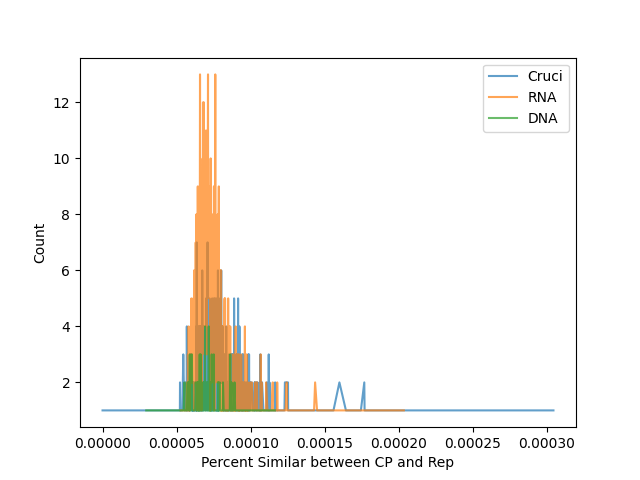
\includegraphics[scale = 0.6]{KmerSimilarityCpRep.png}
    \caption{The figure shows the distributions of the percentages of similar k-mers between the CP and Rep genes of each genome in the crucivirus dataset, RNA virus dataset, and DNA virus dataset. }
\end{figure}
\textbf{Figure 4.} All three virus types have right-skewed distributions with most of the genomes having a percentage of the similarity of CP and Rep between 5.0e-05 and 1.2e-04. The three viruses have similar peaks, at approximately 7.19e-05. Because of this, we are not able to predict the relative locations in time that the three viruses appeared. Crucivirus has the most extensive range from 0 to 3.0e-04 compared to RNA virus and DNA virus, which have ranges 5.0e-05 to 2.0e-04 and 2.8e-05 to 1.1e-04 respectively. This means that crucivirus has the greatest diversity in its genomes and in the time that the CP and Rep genes of the genomes have been in the same virus. This suggests that crucivirus has a relatively longer history because more of its genomes have a higher percentage of similar k-mers between CP and Rep. However, the dataset that we currently use is too small to be more certain. However, because some crucivirus genomes have almost 0.0 percentage of similar k-mers between CP and Rep, we may infer that crucivirus is still showing significant changes in their genetic composition. This may indicate relatively higher rates of mutations for crucivirus as well as more horizontal genetic transfers.

\subsection{Comparison of K-mer between Genomes}

The frequency of k-mer can be used to identify horizontal genetic transfers between genomes. When a k-mer has an overrepresentation in one genome but appears less frequently in another, we can predict that a horizontal genetic transfer has occurred and the direction of the transfer from the first genome to the second. We want to identify horizontal genetic transfers between DNA and crucivirus. Using the two datasets for DNA virus and crucivirus, we found the percentage of matching k-mer between each pair of DNA virus and crucivirus. We selected the pairs with the least similarity and greatest similarity and found the composition of shared k-mer sequences for each pair. This allows us to distinguish the significant frequency of k-mer from the other k-mers. The k-mers that appeared a great number of times may have been transferred from the DNA virus to the crucivirus or vice versa.

\begin{figure}
    \centering
    \textbf{Percentage of Similar K-mer Between Crucivirus and DNA pairs}
    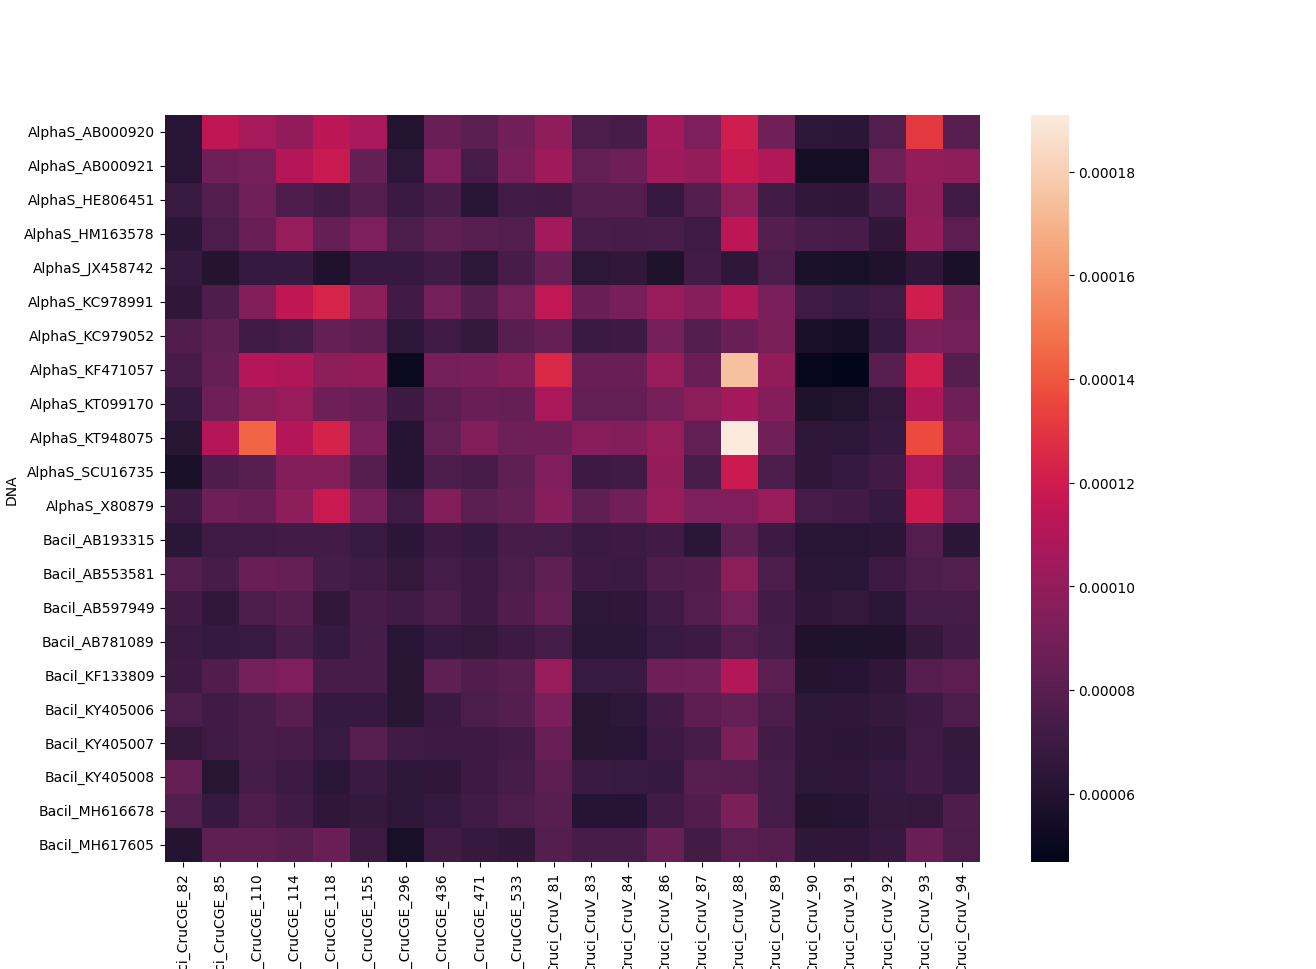
\includegraphics[scale = 0.3]{ComparisonBetweenDNAandCruci.png}
    \caption{The figure shows the percentages of similar k-mers between every possible pair of Crucivirus and DNA virus from the two datasets of 22 crucivirus and 22 DNA virus. The percentages are represented as color within the range of the color bar, with lighter color representing higher percentage and darker color representing lower percentage.}
\end{figure}
\textbf{Figure 5.} Each cell of the heatmap represents the percentage of similar k-mers between a pair of DNA viruses and crucivirus. Most cells are shades of purple and pink, which represent percentages below 1.2e-04. 

Pairs that have high percentages of similar k-mers are 
\begin{itemize}
    \item \texttt{Cruci\_CruV\_88} and \texttt{AlphaS\_KF471057}
    \item \texttt{Cruci\_CruV\_88} and \texttt{AlphaS\_KT948075}
\end{itemize}

Pairs with low percentages of similar k-mers are

\begin{itemize}
    \item \texttt{Cruci\_CruCGE\_296} and \texttt{Bacil\_MH617605}
    \item \texttt{Cruci\_CruV\_87} and \texttt{Bacil\_AB193315}
\end{itemize}

\begin{figure}
    \centering
    \textbf{Count of Shared K-mers between \texttt{Cruci\_CruV\_88} and \texttt{Alpha\_KF471057}}
    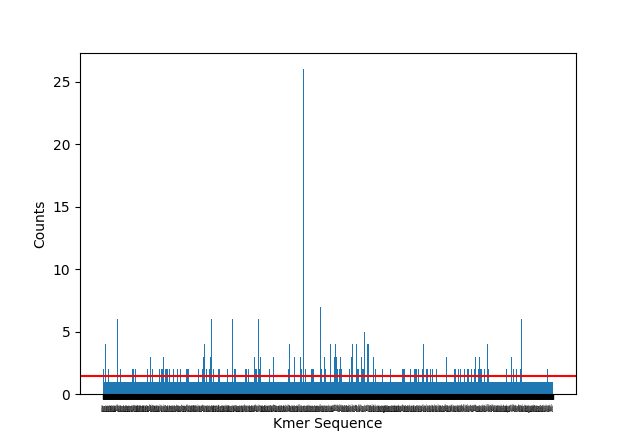
\includegraphics[scale = 0.5]{ComparisonBetweenCruci88DNAKF47105.png}
    \caption{The y-axis shows the number of times that each shared k-mer, shown in the x-axis, appeared in both genomes.}
\end{figure}

\begin{figure}
    \centering
    \textbf{Count of Shared K-mers between \texttt{Cruci\_CruV\_88} and \texttt{AlphaS\_KT948057}}
    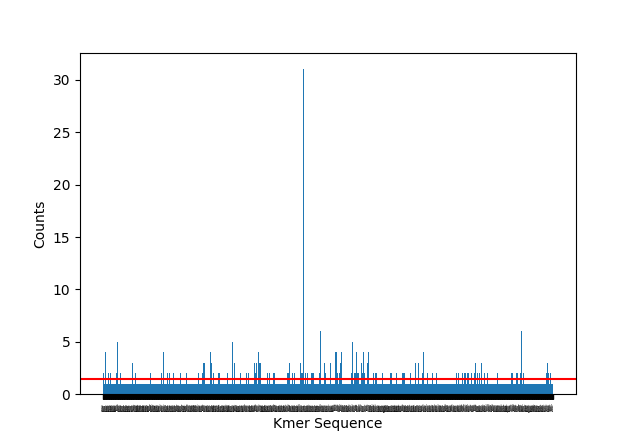
\includegraphics[scale = 0.5]{ComparisonBetweenCruci88DNAKT04807.png}
    \caption{The y-axis shows the number of times that each shared k-mer, shown in the x-axis, appeared in both genomes.}
\end{figure}

\begin{figure}
    \centering
    \textbf{Count of Shared K-mers between \texttt{Cruci\_CruCGE\_296} and \texttt{Bacil\_MH617605}}
    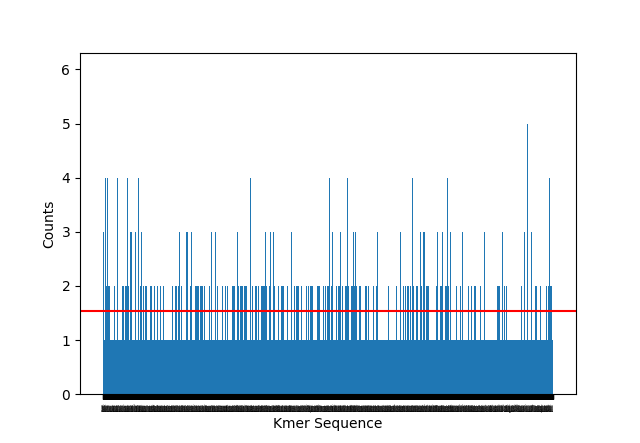
\includegraphics[scale = 0.5]{ComparisonBetweenCruci296DNAMH617605.png}
    \caption{The y-axis shows  the number of times that each shared k-mer, shown in the x-axis, appeared in both genomes.}
\end{figure}

\begin{figure}
    \centering
    \textbf{Count of Shared K-mers between \texttt{Cruci\_CruV\_87} and \texttt{Bacil\_AB193315}}
    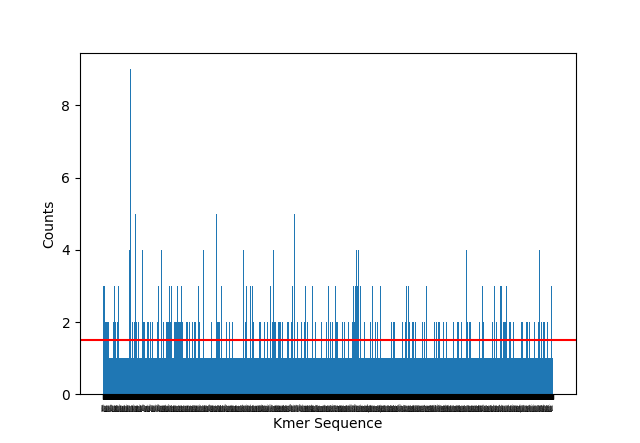
\includegraphics[scale = 0.5]{ComparisonBetweenCruci87DNAAB19331.png}
    \caption{The y-axis shows the number of times that each shared kmer, shown in the x-axis, appeared in both genomes.}
\end{figure}
There are clear differences in the graphs between genome pairs with low similarity and genome pairs with high similarity. Genome pairs with high similarities have one k-mer that has significant overrepresentation. \textbf{Figure 6.} \texttt{Cruci\_CruV\_88} and \texttt{AlphaS\_KF471057} have a count of 26 for AAAAAAA and an average count of 1.47. The large difference between the count of 26 and the average count shows the significance of AAAAAAA in the overall distribution of k-mers. \textbf{Figure 7.} Similarly, \texttt{Cruci\_CruV\_88} and \texttt{AlphaS\_KT948057} have an overrepresentation of 31 for AAAAAAA, which differentiates greatly from the average count of 1.47. 

On the other hand, genome pairs with low similarities have a more even number of counts. \textbf{Figure 8.} \texttt{Cruci\_CruCGE\_296} and \texttt{Bacil\_MH617605} have an average count of 1.54. The k-mer with the highest count is TGGATTC and the count is 5. \textbf{Figure 9.} \texttt{Cruci\_CruV\_87} and \texttt{Bacil\_AB193315} have an average count of 1.49. The highest count of 9 is at AAAGAAA. 

The overrepresentation of AAAAAAA for the genome pairs with high percentages of k-mer similarities suggests that there might be horizontal genetic transfer within the genome pairs. 

A further application can include distinguishing the counts of k-mers for each genome from the total counts to predict the direction of the genetic transfers.

\section{Limitation}

One limitation of our project is the varying sizes of the datasets. RNA has a dataset of 1626 genomes while the crucivirus dataset only has 885 genomes and the DNA dataset has 316 genomes. While we used percentages to cancel out the differences in data size, this still limits the confidence in our results. DNA only has a small dataset so our results for DNA may not be as reliable as our results for RNA or crucivirus. The datasets, even the dataset for RNA, are still too small for us to generalize our results on the population of viruses. For example, we used the dataset of crucivirus genomes to check the accuracy of our genome sense predictions. A larger dataset may result in a different accuracy. For future research, we can apply these analyses to larger datasets. Furthermore, the limitations of my laptop, on which we did the analyses, restricted the size of the data that we can test. Large datasets cause some of our programs to either terminate or take a long time to run. For example, we originally hoped to test pairwise comparison analysis on the entire crucivirus CP and Rep genes datasets. However, the datasets for CP and Rep are each more than 800 genomes long and we estimated that it would take more than an hour or even two hours to complete running our program. Because of this, we had to limit the datasets to only the first 22 genes of CP and Rep based on the dataset of crucivirus genomes that they belong to. If we want to conduct our analyses on larger datasets, we will have to use more powerful computers. 

The genome sense prediction program we made has only 70.01\% accuracy. Excluding the 119 genomes that we classified as unexpected, we have 155 genomes predicted wrong. This makes the accuracy of approximately 81.23\%. A more preferred accuracy that gives us high confidence in our program is 95\% or greater. A future application could be to improve upon the program. In the current program, we only consider horizontal genetic transfer as a factor that influences the predictions other than codon-ending preference. We can look deeper into other factors that determines a genome's sense. By taking into account more factors, we can improve the accuracy of the program.

Finally, we do not have too much discussion on the dendrograms. Dendrograms are useful techniques to visualize and predict the phylogenetic tree and evolution of organisms and the genetic materials of organisms. However, I still haven't figured out how Scipy, the Python library that I used to draw the dendrograms, defines dendrogram clusters. The lack of discussion in Figure 3., the figure with the two dendrograms for pairwise comparison, causes us to miss potentially useful information on the evolution of capsid and replication genes of crucivirus and their relationship with each other, such as whether they evolved separately or are mostly similar in their genetic mutations. 

\section{Conclusion}
The discovery of crucivirus overturned previous beliefs on viruses and their evolution. However, the connection between crucivirus and the RNA- or DNA-only viruses is still a mystery. This project investigates the use of alignment-free analyses on unveiling the evolution of crucivirus and the relationships between crucivirus, DNA virus, and RNA virus. We employed four alignment-free analyses: genome sense prediction, pairwise comparison, k-mer similarity between capsid and replication genes, and comparison of k-mer between genomes. Genome sense prediction helped us find crucivirus genomes that have undergone horizontal genetic transfer recently and comparison of k-mer between genomes allowed us to identify possible sequences in the viruses' nucleic acid that were results of horizontal genetic transfers. K-mer similarity between CP and Rep genes helped us predict the origin of the capsid gene (whether the capsid gene is grabbed from an RNA virus or had existed in the virus for a long period of time). Pairwise comparison helped us predict the phylogenetic tree of capsid and replication genes and their relationship. 

alignment-free analysis shines a new light on the study of crucivirus and viral evolution. It brings useful insights that may help scientists uncover the truth about the history of one of the most abundant and important components on Earth.

\section{Acknowledgements}
I would like to thank my mentor, Dr. Ignacio de la Higuera, who guided and supported me throughout this project. I would also like to thank the Institute for Computing in Research for giving me this opportunity.

% Include references
\insertbibliography{References}
[1] Crewe, G. (2023). The Importance Of Viruses I Oxford Open Learning. Ool.co.uk. https://www.ool.co.uk/blog/the-importance-of-viruses/

[2] Molecular Expressions Cell Biology: Virus Structure. (2022). Fsu.edu. https://micro.magnet.fsu.edu/cells/virus.html

[3] de la Higuera I, Kasun GW, Torrance EL, Pratt AA, Maluenda A, Colombet J, Bisseux M, Ravet V, Dayaram A, Stainton D, Kraberger S, Zawar-Reza P, Goldstien S, Briskie JV, White R, Taylor H, Gomez C, Ainley DG, Harding JS, Fontenele RS, Schreck J, Ribeiro SG, Oswald SA, Arnold JM, Enault F, Varsani A, Stedman KM. Unveiling Crucivirus Diversity by Mining Metagenomic Data. mBio. 2020 Sep 1;11(5):e01410-20. doi: 10.1128/mBio.01410-20. PMID: 32873755; PMCID: PMC7468197.

[4] (2014). Extreme Virus Lab. Extreme Virus Lab. https://www.extremeviruses.org/crucivirusesrdhvs

[5] Bernard G, Chan CX, Chan YB, Chua XY, Cong Y, Hogan JM, Maetschke SR, Ragan MA. Alignment-free inference of hierarchical and reticulate phylogenomic relationships. Brief Bioinform. 2019 Mar 22;20(2):426-435. doi: 10.1093/bib/bbx067. PMID: 28673025; PMCID: PMC6433738.

[6] Crespo-Bellido, A., and Duffy, S. (2022). Strand-Specific Patterns of Codon Usage Bias Across Cressdnaviricota. Front. Virol. 2, 1–17. doi: 10.3389/fviro.2022.899608.
‌
\end{document}
